\documentclass[english,11pt]{article}
\usepackage[T1]{fontenc}
\usepackage[latin9]{inputenc}
\usepackage{babel}
\usepackage{array}
\usepackage{hyperref}
\usepackage{url}
\usepackage[colorinlistoftodos]{todonotes}
\usepackage{booktabs}
\usepackage{rotating}
\usepackage[margin=.75in]{geometry}
\usepackage{siunitx}
\usepackage{color}

\newcommand*\rot{\rotatebox{0}}
\newcolumntype{L}[1]{>{\raggedright\arraybackslash}m{#1}}
\newcolumntype{M}[1]{>{\centering\arraybackslash}m{#1}}

\begin{document}

\title{The Intrinsic Brain Activity Test Re-test Neuroimaging Dataset}

\author{R. Cameron Craddock\textsuperscript{1,2} \and  
        Jonathan Lisinski\textsuperscript{3} \and 
        Stephen LaConte\textsuperscript{3,4,5,6$\dagger$}}

%\author{Firstname Lastname\textsuperscript{1}, Firstname
%Lastname\textsuperscript{2{*}}}

\maketitle

\textsuperscript{1}Center for Advanced Brain Imaging, Nathan Kline Institute for Psychiatric Research,      
    Orangeburg, NY, USA
\textsuperscript{2}Center for the Developing Brain, Child Mind Institute, New York, NY, USA
\textsuperscript{3}Virginia Tech Carilion Research Institute, Roanoke, VA, USA
\textsuperscript{4}School of Biomedical Engineering and Sciences, Virginia Tech and Wake Forest University,
    Blacksburg, VA, USA
\textsuperscript{5}Department of Emergency Medicine, Virginia Tech Carilion School of Medicine, Roanoke, VA, USA
\textsuperscript{6}Department of Radiology, Virginia Tech Carilion School of Medicine, Roanoke, VA, USA
\textsuperscript{$\dagger$}Corresponding author: Stephen LaConte (slaconte@vtcri.vt.edu)


\begin{abstract}
\textcolor{blue}{This is a manuscript template for Data Descriptor submissions to \emph{Scientific
Data} (http://www.nature.com/scientificdata). The abstract must be
no longer than 170 words, and should succinctly describe the study,
the assay(s) performed, the resulting data\todo{finish abstract}, and the reuse potential,
but should not make any claims regarding new scientific findings.
No references are allowed in this section.}
\end{abstract}

\section*{Background \& Summary}

\textcolor{blue}{(700 words maximum) An overview of the study design, the assay(s)
performed, and the created data, including any background information
needed to put this study in the context of previous work and the literature.
The section should also briefly outline the broader goals that motivated
the creation of this dataset and the potential reuse value. We also
encourage authors to include a figure that provides a schematic overview
of the study and assay(s) design. This section and the other main
body sections of the manuscript should include citations to the literature
as needed \cite{cite1, cite2}. References should be included within the 
manuscript file itself as our system cannot accept BibTeX bibliography files. 
Authors who wish to use BibTeX to prepare their references should therefore 
copy the reference list from the .bbl file that BibTeX generates and paste it 
into the main manuscript .tex file (and delete the associated 
\textbackslash{}bibliography and \textbackslash{}bibliographystyle commands).}

\textcolor{green}{357 words of 700 maximum}

Human brain function is divided amongst several intrinsic connectivity networks (ICN), which are constellations of brain regions that are synchronized by spontaneous brain activity. These networks have been observed to be consistent across individuals, scanning sessions and experimental paradigms. The persistence of these networks across rest and task conditions has led many to beleive that they play a central role in human cognition. Importantly the interaction between ICNs has been shown to be linked to inter-individual variability in task performance and imbalances in these interactions are beleived to underly mental disorders such as depression, ADHD, anxiety, and many more. Unfortunately, current experimental methodologies and computational tools are insufficient for fully exploring the interactions between networks and new methods need to be developed to understand this phenomena. 

The Intrinsic Brain Activity Test - Retest (IBA-TRT) dataset was designed as a validation dataset for developing methods for modelling the interactions between ICNs both at rest and during task performance. The study employed an intra- and inter- session test-retest design in which two 10-minute resting state scans, and two 6.5-minute multi-source interference task (MSIT) \cite{bush} scans were acquired in each of two scanning sessions. The MSIT was chosen since it was explictily designed to robustly activates regions commonly associated with task positive networks and since it robustly deactivates the default network. Thirty-six individuals (18F, 20-48 years old) participated in the first scan, 14 of which (5F, 20-40 years old) returned two to six months later for a followup scan. 

The IBA-TRT is a part of the Consortium for Reliability and Reproducibility (CoRR, \url{http://fcon_1000.projects.nitrc.org/indi/CoRR/html/}), which is an open science resource of publicly shared resting state data for assessing the reliability and reproducibility of resting state fMRI analyses. This is one of 33 datasets that are involved with CoRR that has amassed 5093 datasets from 1629 different subjects. Each of the datasets has a slightly different design, as each one of them was intended for slighly different purpose, but there should be sufficient overlap to aggregate dataset for a very large test-retest analysis. The IBA-TRT dataset is one of two datasets to offer task data, the Nathan Kline Institute test-retest dataset includes visual checkerboard and breath holding tasks. 

\section*{Methods }

\input{demo_table}
\begin{table}[ht!]
\centering
\caption{Image acquisition sequence parameters. Scans were acquired in the order presented.}
\label{tab:rest_scan_params}

\small

\begin{tabular}{L{2in}M{1.5in}M{1.5in}M{1.5in}}

\toprule%

& {\bfseries Anatomical}
& {\bfseries Rest (1 \& 2)}
& {\bfseries MSIT (1 \& 2)} \\

\midrule

Sequence & 3D magnetization prepared rapid acquired gradient echo (MPRAGE) & gradient-echo echo-planar-imaging (GE-EPI)  & gradient-echo echo-planar-imaging (GE-EPI) \\
Flip angle & $8^\circ$ & $90^\circ$ & $90^\circ$ \\
Inversion time (TI) & 900 \si{\milli\second} & N/A & N/A \\
Echo time (TE) & 3.02 \si{\milli\second} & 30 \si{\milli\second} & 30 \si{\milli\second} \\ 
Repetition time (TR) & 2600 \si{\milli\second} & 1750 \si{\milli\second} & 1750 \si{\milli\second} \\
Bandwidth per voxel (readout) & 130 \si{\hertz} & 2442 \si{\hertz} & 2442 \si{\hertz} \\
Parallel acceleration & GRAPPA $\times 2$ & None & None \\
Partial fourier & 6/8 phase \& 7/8 slice & Off & Off \\
Number of Slices & 176 & 29 & 29 \\
Slice orientation & saggital & axial-oblique & axial-oblique \\
Slice phase encoding direction & anterior to posterior & anterior to posterior & anterior to posterior \\
Slice acqusition order & sequential ascending & interleaved ascending & interleaved ascending \\
Slice thickness & 1.0 \si{\milli\meter} & 3.6 \si{\milli\meter} & 3.6 \si{\milli\meter} \\
Slice gap & 0.0 \si{\milli\meter} & 0.36 \si{\milli\meter} & 0.36 \si{\milli\meter} \\
Field of view (FOV) & $256 \times 256$ \si{\milli\meter\squared} & $220 \times 220$ \si{\milli\meter\squared} & 
    $220 \times 220$ \si{\milli\meter\squared} \\
Acquisition matrix & $256 \times 256$ & $64 \times 64$ & $64 \times 64$ \\
Slice in-plane resolution & $1.0 \times 1.0$ \si{\milli\meter\squared} & $3.44 \times 3.44$ \si{\milli\meter\squared} &
    $3.44 \times 3.44$ \si{\milli\meter\squared} \\
Number of measurements & 1 & 343 & 224 \\
Acquisition time (TA) & 4 \si{\minute} 38 \si{\second} & 10 \si{\minute} 4 \si{\second} &
    6 \si{\minute} 36 \si{\second} \\ 

\bottomrule    
\end{tabular}

\end{table}

\subsection*{Participants}

\subsection*{MRI Scanning}

All scans were acquired using one of three identical 3T Siemens TIM Trio scanners (Siemens Medical Solutions USA; Malvern, PA) at the Baylor College of Medicine Human Neuroimaging Lab in Houston, TX. Each scanner was equipped with 40 \si{\milli\tesla\per\meter} gradients, 8 receive channels, and a 12-channel head matrix. Visual stimuli were directly projected onto a screen at the head-end of the scanner bore and were visible to participants through a mirror affixed to the head coil\todo{do we need luminescence and/or visual angle measurements?}. Responses to task conditions (during the MSIT) were recorded with a linear four-button fiber optic button box (Current Designs, Inc.; Philadelphia, PA) in the participant's dominant hand (all were right handed). Participants were in constant contact with the scanner operator through a pneumatic head phone and microphone system (Avotec, Inc.; Stuart, FL). 

Each scanning session involved the acquisition of a T1-weighted anatomical image followed by two resting state scans (Rest 1 \& Rest 2), and ended with two acquisitions of the multi-source interference task (MSIT 1 \& MSIT 2). The sequence parameters utilized to acquire each of these scans are detailed in table \ref{tab:rest_scan_params}. The Rest and MSIT scans are described in more detail below.

\subsubsection*{Resting State Scan (Rest)}

The following instructions were read to the participant prior to the first resting state scan: ``Next is a resting state scan.  Please lie quietly with your eyes open and fixate on the fixation cross.  During the scan let your mind wander freely.  Do not perform any sort of mental calculation, memory recall, or other mental tasks.  If you notice yourself focusing on a particular stream of thought, let your mind wander away.  It is important that you remain awake and keep your head still during this scan.  It will last 10 minutes.'' Before the second scan the instructions were: ``We will now perform another resting state scan.  Please remember to lie quietly with your eyes open, fixate on the fixation cross, let your mind wander freely, do not move and do not fall asleep.  The scan will last 10 minutes.''

\subsubsection*{Multi-Source Interference Task (MSIT)}

The MSIT task was programmed in Python using the VisionEGG library\cite{needed} and implements the more recent description of the task by Bush and colleagues\cite{needed}. The MSIT is a block design that begins and ends with 28-second blocks of fixation and involves four 42-second blocks of coherent stimuli interleaved with four 42-second blocks of incoherent stimuli. Each stimuli is presented for 1.75 \si{\second} and involves three numerals, two of which are always the same and one that always differs (target) (see Fig. \ref{fig:msit_stim}). The participant is instructed to press a button on a button box that corresponds to the \emph{value} of the target numeral. During coherent trials, the non-target numerals are always zero and the value of the target numeral corresponds to its position. During incoherent trials, the non-target numerals are non-zero and the target numeral does not correspond to its position. Prior to each run of the MSIT, participants were reminded of the task instructions and asked to respond as accurately and quickly as possible. Each run of the MSIT lasts 6 \si{\minute} and 32 \si{\second}.

\begin{figure}[!ht]
    \centering
    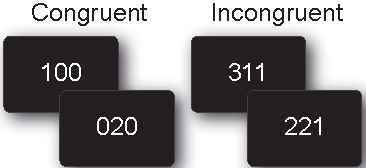
\includegraphics[]{msit_stim2}
    \caption{Example of coherent and incoherent stimuli for MSIT task.}
    \label{fig:msit_stim}
\end{figure}

\textcolor{blue}{This section should include detailed text describing the methods used
in the study and assay(s), and the processing steps leading to the
production of the data files, including any computational analyses
(e.g. normalization, image feature extraction). These methods should
be described in enough detail to allow other researchers to interpret
and repeat, if required, the study and assay(s). Authors are encouraged
to cite previous descriptions of the methods under use, but ideally
the methods descriptions should be complete enough for others to understand
and reproduce the methods and processing steps without referring to
associated publications. In principle, fundamentally new methods should
not be presented for the first time in Data Descriptors, and we may
choose to decline publication of a Data Descriptor until any novel
methods or techniques are published in an appropriate research or
methods-focused journal article.}


\section*{Data Records }

\textcolor{blue}{Please explain each data record associated with this work, including
the repository where this information is stored, and an overview of
the data files and their formats. Each external data record should
be cited using the data citation format explained at the end of this
template.}


\section*{Technical Validation }

\textcolor{blue}{This section presents any experiments or analyses that are needed
to support the technical quality of the dataset. This section may
be supported by up figures and tables, as needed. This is a required
section; authors must present information justifying the reliability
of their data.}


\section*{Usage Notes}

\textcolor{blue}{Brief instructions that may help other researchers reuse these dataset.
This is an optional section, but strongly encouraged when helpful
to readers. This may include discussion of software packages that
are suitable for analyzing the assay data files, suggested downstream
processing steps (e.g. normalization, etc.), or tips for integrating
or comparing this with other datasets. If needed, authors are encouraged
to upload code, programs, or data processing workflows as Supplementary
Information, when they may help others analyze the data.}

\textcolor{blue}{For studies involving privacy or safety controls on public access
to the data, this section should describe in detail these controls,
including how authors can apply to access the data, and what criteria
will be used to determine who may access the data, and any limitations
on data use. }


\section*{Acknowledgements }

\textcolor{blue}{Text acknowledging non-author contributors. Acknowledgements should
be brief, and should not include thanks to anonymous referees and
editors, or effusive comments. Grant or contribution numbers may be
acknowledged. Author contributions Please describe briefly the contributions
of each author to this work on a separate line. }


RCC and SL designed the experiment. RCC and JL collected the data. RCC performed 
quality assessment and validation. RCC, JL, and SL wrote the manuscript.

\section*{Competing financial interests }

The author(s) declare no competing financial interests.


\section*{Figures Legends}

\textcolor{blue}{Figure should be referred to using a consistent numbering scheme through
the entire Data Descriptor. For initial submissions, authors may choose
to supply this document as a single PDF with embedded figures, but
separate figure image files must be provided for revisions and accepted
manuscripts. In most cases, a Data Descriptor should not contain more
than three figures, but more may be allowed when needed. We discourage
the inclusion of figures in the Supplementary Information \textendash{}
all key figures should be included here in the main Figure section. }

\textcolor{blue}{Figure legends begin with a brief title sentence for the whole figure
and continue with a short description of what is shown in each panel,
as well as explaining any symbols used. Legend must total no more
than 350 words, and may contain literature references. }


\section*{Tables}

\textcolor{blue}{Tables supporting the Data Descriptor. These can provide summary information
(sample numbers, demographics, etc.), but they should generally not
be used to present primary data (i.e. measurements). Tables containing
primary data should be submitted to an appropriate data repository. }

\textcolor{blue}{Tables may be provided within the \LaTeX{} document or as separate
files (tab-delimited text or Excel files). Legends, where needed,
should be included here. Generally, a Data Descriptor should have
fewer than ten Tables, but more may be allowed when needed. Tables
may be of any size, but only Tables which fit onto a single printed
page will be included in the PDF version of the article (up to a maximum
of three). }


\section*{Supplementary Information}

\textcolor{blue}{Names and short legends for each supporting file. Supplementary Information
may include code and workflows, media content (images, videos, etc.),
and any other files required to support the data description or to
help others reuse the data. Primary data files should be stored in
an external data repository, not the Supplementary Information section.
In most cases, the Supplementary Information should not contain text
documents or supplemental figures \textendash{} all textual information
and figures that are central to the Data Descriptor should be included
in the main document. The Methods, Technical Validation, and Usage
Notes sections are all of unrestricted length. }


\bibliography{vtcri_trt}{}
\bibliographystyle{naturemag}
\end{document}

%\begin{thebibliography}{1}
%\expandafter\ifx\csname url\endcsname\relax
%  \def\url#1{\texttt{#1}}\fi
%\expandafter\ifx\csname urlprefix\endcsname\relax\def\urlprefix{URL }\fi
%\providecommand{\bibinfo}[2]{#2}
%\providecommand{\eprint}[2][]{\url{#2}}

%\bibitem{cite1}
%\bibinfo{author}{Califano, A.}, \bibinfo{author}{Butte, A.~J.},
%  \bibinfo{author}{Friend, S.}, \bibinfo{author}{Ideker, T.} \&
%  \bibinfo{author}{Schadt, E.}
%\newblock \bibinfo{title}{{Leveraging models of cell regulation and GWAS data
%  in integrative network-based association studies}}.
%\newblock \emph{\bibinfo{journal}{Nature Genetics}}
%  \textbf{\bibinfo{volume}{44}}, \bibinfo{pages}{841--847}
%  (\bibinfo{year}{2012}).

%\bibitem{cite2}
%\bibinfo{author}{Wang, R.} \emph{et~al.}
%\newblock \bibinfo{title}{{PRIDE Inspector: a tool to visualize and validate MS
%  proteomics data.}}
%\newblock \emph{\bibinfo{journal}{Nature Biotechnology}}
%  \textbf{\bibinfo{volume}{30}}, \bibinfo{pages}{135--137}
%  (\bibinfo{year}{2012}).

%\end{thebibliography}

\section*{Data Citations}

Bibliographic information for the data records described in the manuscript.


1. Lastname1, Initial1., Lastname2, Initial2., ...\& LastnameN, InitialN. Repository name Dataset accession number or DOI (YYYY).

\end{document}

